\section{Implementace prototypu herních mechanik}

\subsection{Architektura a účel prototypu}

V tomto prototypu jsem implementoval základní herní mechaniky nezbytné pro provádění simulací a shromažďování dat, na jejichž základě budou v dalších fázích výzkumu rozšiřovány typy jednotek a budov a upravovány jejich statistiky. Architektura prototypu je založena na čtyřech klíčových třídách \ref{diagram_trid}, které zajišťují funkčnost herního cyklu a interakci mezi herními objekty:

\begin{itemize}
    \item \texttt{SpravceHry}: Centrální řídicí prvek, který spravuje průběh hry, střídání hráčů a implementuje základní umělou inteligenci. Zajišťuje koordinaci mezi ostatními třídami.
    \item \texttt{Hrac}: Reprezentuje jednotlivého hráče ve hře. Spravuje jeho ekonomiku (suroviny), vlastněné jednotky a budovy.
    \item \texttt{Jednotka}: Představuje herní jednotky s atributy jako útok, obrana, životy a pohyb.
    \item \texttt{Budova}: Reprezentuje hráčské budovy, které v prototypu primárně slouží k produkci surovin. Jejich implementace je v prototypu zjednodušená, spíše abstraktní.
\end{itemize}

Účelem tohoto prototypu je získat funkční základ pro simulace herních scénářů s různými konfiguracemi jednotek a budov. Získaná data poslouží k informovanému návrhu nových typů jednotek a budov a k úpravě jejich statistik pro dosažení vyvážené hratelnosti v plné verzi hry.

\begin{figure}
  \centering      % vycentrovat
  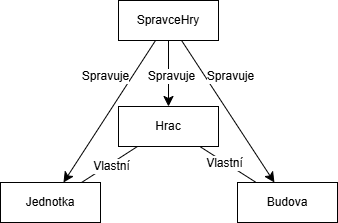
\includegraphics[scale=0.8]{obr/tridy.png} % soubor + měřítko (scale)
  \caption{Zjednodušený diagram tříd.} % popis obrázku
  \label{diagram_trid} % definice odkazu na obrázek (pro \ref{})
\end{figure}

\subsection{Třída \texttt{SpravceHry}}

Třída \texttt{SpravceHry} je hlavním řídicím prvkem celé hry. Zajišťuje koordinaci všech částí systému, spravuje průběh jednotlivých tahů a obsahuje také jednoduchou implementaci umělé inteligence ovládající hráče pro účely testování. Jedná se o centrální bod, který propojuje třídy \texttt{Hrac}, \texttt{Jednotka} a \texttt{Budova} a zabezpečuje jejich souhru v rámci herního cyklu.

Hlavní úlohy třídy zahrnují: 
\begin{itemize} 
    \item aktualizaci stavu hry v jednotlivých tazích, 
    \item správu střídání hráčů a ukončení hry při splnění podmínky vítězství, 
    \item rozhodování AI o pohybu a útocích jednotek. 
\end{itemize}

\paragraph{Aktualizace hry.}
Před začátkem hry je pomocí \texttt{inicializace\_hry} vytvořeno počáteční rozestavení hráčů včetně jejich základen a startovní ekonomiky (\texttt{startovni\_domek}).

Pomocí metody \texttt{aktualni\_hrac} se zjistí, který hráč je aktuálně na tahu. Střídání hráčů je zajištěno metodou \texttt{dalsi\_hrac}, která po odehrání všech hráčů zvyšuje číslo kola.

Při splnění podmínky vítězství (např. zničení základny) je hra ukončena metodou \texttt{konec}, která zaznamená výsledek a ukončí herní cyklus.

\paragraph{Provedení tahu.}
Metoda \texttt{proved\_tah} spravuje celý tah aktuálního hráče, včetně aktualizace surovin, vyhodnocení údržby jednotek a provedení akcí AI.

Metoda \texttt{kontrola\_bojeschopnosti} ověřuje, zda hráč po ztrátách ještě má bojeschopné jednotky.

\paragraph{Rozhodování AI.}  
Jednoduchá AI, implementovaná metodami \texttt{ai\_tah}, \texttt{ai\_pohyb\_a\_utok} a \texttt{stavba\_a\_verbovani\_ai}, vyhodnocuje akce jednotek hráče v daném tahu. Jednotky nejprve útočí na nejbližšího nepřítele v dosahu, pokud je k dispozici, nebo hledají nepřátelské jednotky v okolí jednoho kroku.Pokud ani tak nedosáhnou, posouvají se směrem k nepřátelské základně. Po pohybu jednotek, na základě aktuálního zisku surovin, AI rozhoduje o stavbě nových budov nebo verbování nových jednotek.

\paragraph{Verbování a Stavba}
Nové jednotky jsou vytvářeny metodou \texttt{verbovani}, která ověřuje podmínky a najde volné místo v okolí základny. 

Stavba budov probíhá obdobně metodou \texttt{stavba\_budovy}, pouze je zde na pevno daná pozice, jelikož umístění budov neberu v prototypu v potaz, pracuji 
s nimi jako s abstraktními.

\paragraph{Souboje}
Metoda \texttt{vyhodnot\_souboj} řeší útok jednotky na protivníka, včetně protiútoku a odstranění padlých jednotek. Pokud padne základna, hra je ukončena metodou \texttt{konec}.


\subsection{Třída \texttt{Hrac}}

Třída \texttt{Hrac} reprezentuje jednotlivého hráče ve hře. Uchovává jeho jméno, seznam jednotek a budov, dostupné suroviny. Hlavní odpovědností třídy je správa ekonomiky hráče, zejména manipulace se surovinami, zpracování údržby jednotek a vyhodnocení následků nedostatku zdrojů.

Hlavní úlohy třídy zahrnují: 
\begin{itemize} 
    \item správu zásob surovin a jejich změn, 
    \item evidenci vlastněných jednotek a budov, 
    \item zajištění výroby surovin budovami, 
    \item řešení údržby jednotek a následků nedostatku surovin. 
\end{itemize}

\paragraph{Práce se surovinami.}
Třída umožňuje přidávat nové suroviny pomocí metody \texttt{pridej\_suroviny} a odebírat suroviny pomocí \texttt{odecti\_suroviny}. Při odečítání je kontrolováno, zda má hráč dostatek požadovaných zdrojů.

\paragraph{Správa ekonomiky a údržby.}
Každé kolo může hráč získat nové suroviny produkované budovami prostřednictvím metody \texttt{zisk\_z\_budov}. Údržba jednotek je řešena metodou \texttt{zpracuj\_udrzbu}, která odečítá příslušné množství surovin. Pokud hráč nemá dostatek zdrojů, všechny jeho jednotky utrpí ztrátu životů.

\paragraph{Nedostatek jídla.}
Konkrétním případem správy ekonomiky je hladovění jednotek, implementované metodou \texttt{zpracuj\_nedostatek\_jidla}. Pokud hráč nemá dostatek jídla, jeho jednotky ztrácejí životy.


\subsection{Třída \texttt{Jednotka}}

Třída \texttt{Jednotka} reprezentuje jednu funkční jednotku ve hře. Její hlavní úlohou je definovat chování jednotky v rámci herního světa, včetně pohybu, boje a interakce s herním prostředím.

Hlavní úlohy třídy zahrnují:
\begin{itemize}
    \item uchovávání atributů jednotky (typ, pozice, statistiky, cena, vlastník),
    \item výpočet možných pohybů na základě rychlosti a terénu,
    \item realizaci pohybu na zvolenou cílovou pozici,
    \item vyhledávání nepřátelských jednotek v dosahu útoku,
    \item provádění útoku na nepřátelské jednotky a přijímání protiútoků,
    \item správu životů a mechanismus zániku jednotky.
\end{itemize}

\paragraph{Pohyb.}
Metoda \texttt{vypocet\_moznych\_pohybu} na základě aktuální pozice, rychlosti jednotky a typu terénu na herní mapě určuje všechny dosažitelné polohy. Při výpočtu zohledňuje překážky, jako je voda nebo přítomnost jiných jednotek. Metoda \texttt{proved\_pohyb} následně aktualizuje pozici jednotky, pokud je cílová pozice v seznamu možných pohybů.

\paragraph{Boj.}
Metoda \texttt{najdi\_cile\_v\_dosahu} prozkoumá okolí jednotky a vrátí seznam nepřátelských jednotek, které se nacházejí v jejím dosahu útoku. Samotný útok je realizován metodou \texttt{proved\_utok}, která sníží životy napadené jednotky na základě rozdílu mezi útočnou silou útočníka a obranou bránícího se, s případnými modifikátory terénu. Metoda \texttt{proved\_protiutok} umožňuje bránící se jednotce odpovědět na útok, pokud je útočník v jejím dosahu.

\subsection{Třída \texttt{Budova}}
Třída \texttt{Budova} obecně reprezentuje strukturu vlastněnou hráčem, která plní specifickou funkci v rámci hry. Může se jednat o budovy produkující suroviny, obranné stavby nebo jiné speciální budovy. Třída uchovává informace o typu budovy, její pozici na mapě, vlastníkovi, životech, obraně, produkci surovin a ceně za postavení.

Hlavní úlohy třídy zahrnují:
\begin{itemize}
    \item uchovávání atributů budovy (typ, pozice, vlastník, životy, obrana, produkce, cena),
    \item generování surovin.
\end{itemize}

\paragraph{Produkce surovin.}
Pokud je budova určena k produkci surovin, slovník \texttt{produkce} definuje typy surovin a jejich množství, které budova vyprodukuje za jedno herní kolo. Metoda \texttt{generuj\_suroviny} vrací tento slovník, čímž umožňuje hráči získávat zdroje.

\paragraph{Umístění.}
V tomto prototypu je pozice budovy pevně daná při jejím vytvoření a nelze ji měnit. Metoda pro stavbu budovy ve třídě \texttt{SpravceHry} zajišťuje její umístění na předdefinovanou pozici. V prototypu budovy neinteragují s pohybem jednotek ani mezi sebou, takže jejich přesné umístění nemá funkční dopad. 

\paragraph{Speciální funkce a blokování cesty.} Budovy mají v prototypu implementovanou pouze schopnost generovat suroviny. Jejich speciální schopnosti a schopnost blokovat cestu jsem se rozhodl implementovat až v rámci celé hry.